\subsection{Setup}
The next question is whether the implemented pipeline can run on realistic embedded hardware, not only on a powerful desktop computer. This is important because the goal of the system is practical deployment on autonomous marine robots, where compute power, memory, and scheduling behaviour are limited. The setup used for the results therefore represents a normal constrained SBC platform with standard OS settings.
\\ \\
All results presented in this work were produced on a standard Raspberry Pi 4 Model B, shown in Figure \ref{fig:results-setup-rpi4}. The system used the regular quad-core ARM Cortex-A72 processor with 4 CPU cores running at $1.5\,\mathrm{GHz}$ and $4\,\mathrm{GB}$ of RAM. The software setup was a fresh Ubuntu 24.04 LTS installation with Linux kernel 6.8, the default EEVDF kernel scheduler, and ROS2 Jazzy as the middleware layer. No special real-time kernel, manual CPU pinning, overclocking, or custom scheduler configuration was used. The experiments therefore represent the behaviour of the implemented system on a normal embedded SBC setup with standard OS settings.
\\ \\
This setup is deliberately simple. If the system can generate stable maps, extract useful landmarks, and maintain real-time performance on this platform without special tuning of the OS, then the implementation is more relevant for practical embedded deployment.
\begin{figure}[H]
    \centering
    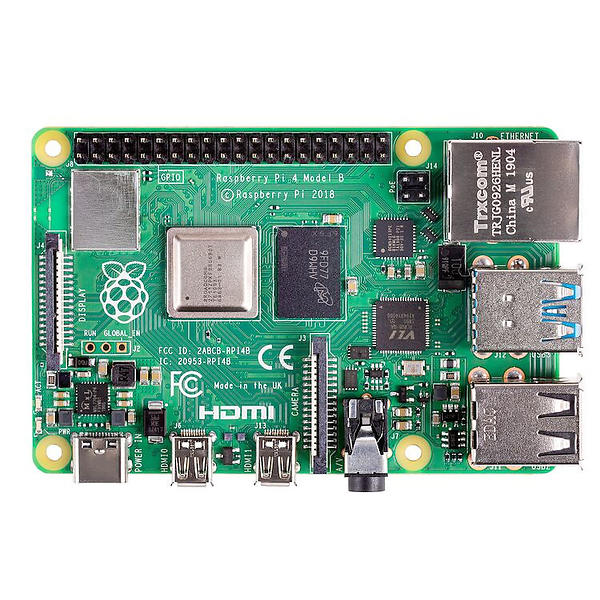
\includegraphics[width=0.7\linewidth]{Pictures/Results/Setup/RPI4.jpg}
    \caption{Picture of Raspberry Pi 4 Model B.}
    \label{fig:results-setup-rpi4}
\end{figure}
